\section{Design Validation}
\label{sec:fdsp-pd-validation}


This section summarizes the most important sets of measurements, completed, ongoing, and planned, that validate the \dword{pds} design. 


\subsection{Photosensors and Active Ganging}
\label{sec:pds-valid-ganging}

As described in Section~\ref{sec:pds-design-ganging}, the active ganging of \dwords{sipm} aims to increase the active photo-detecting area while keeping the number of readout channels at a reasonable number. 
Several active ganging detectors were designed and tested during 2017-2018. 
The systems were based on an active summing node mounted near the photosensors in the \lar. Several incarnations of the cold summing node were designed and tested using SensL and Hamamatsu \dwords{sipm}, 
as were several types of operational amplifiers.
Some of these designs were tested and validated in the \dword{sarapu} prototype measurements.
We describe here only the most recent design that demonstrated that 48 Hamamatsu \dwords{mppc} in the baseline design can be ganged together on a single differential output with excellent signal performance, low noise, and low power dissipation.

Figure~\ref{fig:fig-pds-gang-1} (left) shows a matrix array of 72 \dwords{mppc} organized as 12 rows of six  13360-6050VE \dwords{mppc} each. 
The six \dwords{mppc} per row are connected in parallel, giving a total output capacitance of \SI{7.8}{nF}. The 12 rows are connected to the summing node of an operational amplifier, THS4131, as illustrated in Figure~\ref{fig:fig-pds-gang-1} (right). 
Since the DUNE baseline design is based on 48 \dwords{mppc}/\dword{xarapu} module, only eight rows of six \dwords{mppc} were used for the tests. 
The performance of the cold summing electronics was done by illuminating the \dword{mppc} array with an LED and digitizing the output with a high-speed oscilloscope and with the \dword{ssp} readout electronics (see 
Section~\ref{sec:valid-pdsp}).

As shown in Figure~\ref{fig:fig-pds-gang-2-3}~(left), the mean signal has a rise time of \SI{60}{ns} and a recovery time of \SI{660}{ns}, well within the DUNE \dword{pd} specifications.

\begin{dunefigure}[Photosensors signal ganging scheme]
 {fig:fig-pds-gang-1}
 {Summing board with a total of 72 \dwords{mppc} used to demonstrate the optimal combination of passive and active ganging with 48 Hamamatsu \SI{6}{mm}$\times$\SI{6}{mm} \dwords{mppc} (left).  Schematic of the summing circuit with a THS4131 operational amplifier (right).}
\includegraphics[height=6cm]{graphics/pds_gang_fig1.jpg}
\includegraphics[height=6cm]{graphics/pds_gang_fig2.png}
\end{dunefigure}



\begin{dunefigure}[Photosensors signal ganging with 48 \dshorts{sipm}]
 {fig:fig-pds-gang-2-3}
 {Waveform signal from 48 \dwords{mppc}/ARAPUCA module, summed with the THS4131 operational amplifier and digitized with the \dword{ssp} frontend board (left); histogram of signals with a 47~V bias illustrating the first \phel peak well-separated from the pedestal with an S/N = 9.5 (right).}
\includegraphics[height=5.5cm]{pds-gang-rise_time.jpg}
\includegraphics[height=5.5cm]{graphics/pds-gang48-47v.jpg}
\end{dunefigure}

Figure~\ref{fig:fig-pds-gang-2-3}~(right) shows a histogram of light collection signals from the array for a bias voltage equivalent to \SI{2}{volts} above the mean breakdown voltage. Since there are 48 \dwords{mppc} in the array, and a single common bias, there is a spread in the gains. Even when the Hamamatsu \dwords{mppc} have a small spread in breakdown voltages, it is enough to smear the peaks in the histogram. It is worth distinguishing the difference between noise and gain spread. The circuit noise can be measured as FWHM or RMS around the 0 PE signal (\SI{3.5}{ADC counts} in the figure); the first PE peak is at \SI{33}{ADC counts}, resulting in an optimal signal to noise ratio of about 10.

Since the breakdown voltage of the \dwords{mppc} is provided by the manufacturer for each device, the gain spread can be reduced by picking groups of 48 \dwords{mppc} with similar breakdown values for each module. The differential output of the cold electronics impedance is matched to the readout electronics and able to reject more than \SI{60}{dB} of common mode noise. This is particularly important since the \dwords{mppc} and output wiring are inside a high voltage TPC. The timing properties of the 48 ganged electronics were also measured in LAr using a Am-241 alpha source. 
Figure~\ref{fig:fig-pds-gang-4} shows the time walk for a constant discrimination threshold which, as expected, is not a linear function of the signal height. The error distribution, which is not Gaussian, has a FWHM of \SI{80}{ns}. This value is well within the DUNE specification (Table~\ref{tab:specs:SP-PDS}).

\begin{dunefigure}[Time walk from 48 ganged MPPCs]
 {fig:fig-pds-gang-4}
 {Oscilloscope trace (left) and histogram (right) illustrating time walk from 48 ganged MPPCs measured with the constant discrimination threshold on the SSP board.}
\includegraphics[height=5.5cm]{graphics/pds-gang-time-walk.jpg}
\includegraphics[height=5.5cm]{graphics/pds-gang-time-walk-hist.jpg}
\end{dunefigure}


\textit{\dword{fbk} Sensors} 
\dword{fbk} has published detailed measurements on photosensors developed in collaboration with the DarkSide cryogenic experiment~\cite{Gola:2019idb}. Figure~\ref{fig:fbk-pde-dcr}~(left) shows that the photon detection efficiency of candidates devices as function of wavelength is very well matched to the needs of the \dword{xarapu}.

An extensive program of evaluation of the key performance characteristics is underway by the DUNE \dword{pds} team.
%An extensive program of evaluation is underway for the NUV-HD-SF sensors from \dword{fbk}. 
In the first phase, a sample of (\SI{4}{mm}$\times$\SI{4}{mm}, \SI{40}{$\mu$m} cell-pitch) devices has been tested at INFN-Milano in a dedicated setup optimized for the measurement of very low dark currents. The sensors were operated at \SI{77}{K} and can be biased from \SI{21}{V} (breakdown voltage) up to \SI{31}{V} (maximum overvoltage range at cryogenic temperature is +\SI{10}{V}). The dark count rate at \SI{+4}{V} overvoltage is $\sim$\SI{0.2}{Hz/mm$^2$}, which meets the DUNE requirements (see Figure~\ref{fig:fbk-pde-dcr}~(right)). 
These devices have undergone numerous temperature cycles during the testing with no deterioration in characteristics. Another sample at CSU has undergone more than 50 thermal cycles with no evidence of mechanical failures.  
%The setup at CSU for thermal tests is shown in Figure~\ref{fig:csu-cryocycle}.

\begin{dunefigure}[Performance of candidate FBK \dshorts{sipm}]
 {fig:fbk-pde-dcr}
 {PDE measured at \SI{293}{K} for \dword{fbk} NUV-HD-Cryo and NUV-HD \dwords{sipm} (left); dark count rate for NUV-HD-SF \dwords{sipm} at \SI{77}{K} (right).}
\includegraphics[height=5.5cm]{pds-fbk-pde-pub.png}
\includegraphics[height=4.5cm]{pds-fbk-dcr.png}
\end{dunefigure}


\textit{Mu2e Electronics}
The Mu2e electronics have undergone a series of end-to-end warm and cold tests to demonstrate single-photon sensitivity in various parallel/series ganging and \dword{sipm}/\dword{mppc} configurations. Here we summarize the results with the 72-\dword{mppc} active ganging array described in Section~\ref{sec:pds-valid-ganging}
 at liquid nitrogen temperatures. 
A balun\footnote{A transformer used to convert differential (BALanced) signals to single-ended (UNbalanced) ground referenced signal.} is used to convert from the differential actively-ganged \dword{mppc} array output to the single-ended \dword{feb}.

A trigger allowed data to be collected in time with an LED flasher, with samples taken every 12.5~ns for the length of the readout window ($\sim$3~$\mu$s, in this case). Figure~\ref{fig:pds-board-balun-adc} shows the system used and a histogram of the maximum ADC value during each trigger window. The first peak above zero corresponds to the electronic noise and the second peak corresponds to a one-PE signal. The signal to noise from these tests was measured to be 4, calculated from the ratio of the single photon peak (20~ADC, after subtracting the noise peak) to the spread in the noise ($\sigma_{noise}$ = 5~ADC); this is similar to the value found when using the \dwords{ssp} for readout (S/N~=~5).

\begin{dunefigure}[Readout of 72-\dshort{mppc} active ganging array with the Mu2e electronics readout board]
{fig:pds-board-balun-adc}
{The Mu2e electronics readout board was used to read out a 72-\dword{mppc} active ganging array (V$_b$ = \SI{47.2}{V}) (left). The maximum ADC results are shown, with the first and second peaks representing 0 and 1~\phel signals (right).}
\includegraphics[height=5.2in]{pds-board-balun-adc} 
\vspace{-7.0cm}
\end{dunefigure}


\subsection{Standard ARAPUCA (S-ARAPUCA)}
\label{sec:sarapuca-prototypes}


\subsubsection{Development Prototypes}
\label{sec:valid-initial}

As outlined in Section~\ref{sssec:photoncollectors}, the design for the \dword{sarapu} features a dichroic filter window coated with a wavelength-shifter on the \lar active volume face and a second wavelength shifter coated onto the dichroic filter on the surface inside the cell.  
The proof-of-concept measurements of this design were performed on a small cell with internal dimensions of \SI{3.5}{cm} $\times$ \SI{2.5}{cm} $\times$ \SI{0.6}{cm}, with a window formed from a dichroic filter of  dimensions \SI{3.5}{cm} $\times$ \SI{2.5}{cm} and a wavelength cut-off at \SI{400}{nm}. The external side was coated with \dword{ptp} and the internal side was coated with \dword{tpb}. 
The trapped light was detected by a single \SI{6}{mm} $\times$ \SI{6}{mm} SensL MicroFC-60035C-SMT \dword{sipm}\footnote{SensL \dword{sipm}: \url{http://sensl.com/products/c-series/}}. The cell was exposed to scintillation light produced in pure LAr by an alpha source\footnote{A $^{238}$U-Al alloy in the form of a metallic foil.} that emits three alpha lines with energies of  \SI{4.187}{MeV}, \SI{4.464}{MeV}, and \SI{4.759}{MeV} with relative abundances of 48.9\%, 2.2\%, and 48.9\%. %respectively.
The observed spectrum was fit using the predicted photon yield from the three alpha lines to extract the overall collection efficiency for this configuration of 1.10\%$\pm$0.15\%~\cite{Segreto:2018jdx} for this configuration, consistent with \dword{mc} expectations~\cite{Marinho:2018doi}. This corresponds to a gain in the effective photosensors area of approximately a factor of \num{3.7}. 

A series of subsequent prototypes with filters from different manufacturers, different reflectors, and different dimensions were evaluated with similar results. 

The final set of prototypes prior to \dword{pdsp} were tested in the TallBo facility using an external set of cosmic ray counters as a readout trigger. These consisted of an array of eight \dword{sarapu} cells each with a photon collection area of \SI{80}{cm$^2$}, but the SensL \dwords{sipm} used in previous prototypes were replaced with four \SI{6}{mm} $\times$ \SI{6}{mm} Hamamatsu S13360-6050VE MPPCs. 
Two double-shift light guide modules were also included in the test and served as a reference for the \dword{sarapu} results.

The measured collection efficiency range for the eight ARAPUCA cells was 0.72\% to 0.80\%, with an effective \dword{sarapu} gain of about 4.5 times the photosensor area. These tests demonstrate that the effective area gain is maintained when the area for light collection of the cell is scaled up by almost an order of magnitude.

%%%%%%%%%%%%%%%
\subsubsection{\dword{pdsp}}
\label{sec:valid-pdsp}

The most comprehensive set of data on the \dword{sarapu} will come from the fully instrumented modules in the \dword{pdsp} experiment~\cite{Abi:2017aow} that completed first beam running in November \num{2018}. 
Since \dword{pdsp} will remain filled with \lar for much of the CERN long shutdown, it will provide a long-term cold test of full-scale \dword{pd} modules for the first time, so it may be possible to quantify any deterioration in their performance.

Three prototype photon collector designs are present in \dword{pdsp}: \num{29} double-shift guides, \num{29} dip-coated guides, and two \dword{sarapu} arrays.
The TPC provides precise reconstruction in \threed of the track of any ionizing event inside the active volume, and matching the track with the associated light signal will enable an accurate comparison of the relative photon collection efficiencies of the different \dword{pd} modules. 
The large number of modules and independent channels that record each event can be used to constrain the parameters of the \lar that regulate \dword{vuv} light propagation in the simulation and are poorly determined in the literature. %such as Rayleigh scattering length
In principle, absolute calculations of of the relative and absolute detection efficiencies are possible using \dword{mc} simulations.
The precision of this approach may be limited by the precision of the constraints on the parameters but in any case will result in a consistent simulation constrained by measurements. 


\begin{dunefigure}[Event display from \dshort{pdsp} showing the location of the PD modules]{fig:evtdisplay-pd-protodune}
{Event display from \dshort{pdsp} showing the location of the PD modules on the beam entry side of the TPC. Reconstructed TPC hits from a test beam electron are visible at approximately the same height in the TPC as the \dshort{sarapu} module mounted in APA~3.} 
\includegraphics[height=11.cm]{pds-pdune-display-pd.png}
\end{dunefigure}

\begin{dunefigure}[Full-scale \dshort{sarapu} array installed in \dshort{pdsp} APA~3]{fig:arapuca-protodune}
{Visible in the center of the photograph of APA~3 is the 16-cell \dword{sarapu} array installed in \dword{pdsp}.} 
\includegraphics[height=8.cm]{pds-arpk-apa3_pd.jpg} 
\end{dunefigure}

Figure~\ref{fig:evtdisplay-pd-protodune} shows an event display from \dword{pdsp} overlaid with colored bars indicating the positions of PD modules that are on the beam entry side of the TPC.
Of the two \dword{sarapu} arrays in \dword{pdsp}, the first is installed in the \dword{apa}~3 in the fourth position from the top, near the level at which the beam particles enter this drift volume. This module and the surrounding light guide modules are illuminated with a significant amount of light from each beam particle interaction. This module is visible near the center of the photograph of APA~3 in Figure~\ref{fig:arapuca-protodune}.
The second is installed in  \dword{apa}~6, in the 6th position from the top, in the drift region on the opposite side of the opaque cathode plane, which does not see entering beam particles; this module does not see significant light from beam events (only from showering particles that pass through the cathode), but it observes photons from a large collection of triggered cosmic rays.
 
Each \dword{pdsp} \dword{sarapu} module array is composed of sixteen cells, where each cell is an \dword{sarapu} box with window dimensions of \SI{7.8}{cm}$\times$\SI{9.8}{cm}; half of the cells have twelve \dwords{mppc} installed on the bottom side of the cell and  half have six \dwords{mppc}. 
The \dwords{mppc} used are the Hamamatsu model 13360-6050CQ-SMD, which are functionally the same as the 13360-6050VE used for the ganging tests (Section~\ref{sec:pds-valid-ganging}) and also on some of the light guide bars in \dword{pdsp}, but this model incorporates a package specifically designed for cryogenic operation\footnote{A thin glass window mounted in front of uncoated silicon photosensitive surface, as opposed to the thin coating directly on the silicon for the 13360-6050VE.}. 
The \dwords{mppc} have active dimensions \SI{0.6}{cm}$\times$\SI{0.6}{cm} and account for 5.6\% (\num{12} \dwords{mppc}) or \num{2.8}\% (\num{6} \dwords{mppc}) of the area of the window.
The \dwords{mppc}  are passively ganged together, so that only one readout channel is needed for each \dword{sarapu} grouping of \num{12} \dwords{mppc} (the boxes with six \dwords{mppc} are ganged together to form \num{12}-\dword{mppc} units), so a total of \num{12} channels is required per PD module. 
The total width of a module is \SI{9.6}{cm}, while the active width of an \dword{sarapu} is \SI{7.8}{cm}, the length is the same as the light guide modules ($\sim$\SI{210}{cm})\footnote{Since \dword{pdsp} was constructed, the slot opening in the \dword{apa} opening for \dword{pd} module installation has been enlarged allowing for a module with larger collection area.}.

An \dword{sarapu} array during assembly is shown in Figure~\ref{fig:sarapuca_array_prod}; the array installed in \dword{pdsp} is shown in Figure~\ref{fig:arapuca-protodune}. 
A simulation of the \dword{sarapu} cells, using code that was validated by the earlier prototype measurements (Section~\ref{sec:sarapuca-prototypes}), predicts a photon collection efficiency for the module on the beam side of the cathode of 1.5\%, and for the module on the non-beam side with an optimized configuration, (\num{12} \dwords{sipm} and \dword{ptp} coated on the filter substrate), it could be as high as 3.0\%. A full \dword{sarapu} module with the optimized configuration would have an effective area equivalent to a detector with \SI{36}{cm$^2$} active area with 100\% collection efficiency and produce an average light yield across the TPC of \SI{20}{PE/MeV}.


\begin{dunefigure}[Photograph of an \dshort{sarapu} module prototype assembly]{fig:sarapuca_array_prod}
{\Dword{pdsp} \dword{sarapu} module being assembled in a class 100,000 clean area.  Front face of assembled module (left) shows the 16 coated dichroic filter plates.  Assembly photos show the reflective rear side (top right) and inner coated surface (right bottom) of Vikuiti\texttrademark\ reflective foils.  Note the cutouts in foil for \dword{mppc} active area.}
	\includegraphics[angle=90,width=0.6\columnwidth]{pds-pdune-arapuca-assby}
\end{dunefigure}


As described above, for the \dword{sarapu} modules, the \dwords{sipm} are passively summed in groups of 12 to produce 12 signal channels per module. The 58 light guide-style light collectors each have 12 \dwords{sipm}, which are passively summed in groups of three such that each light guide has four signal channels. 
The unamplified summed analog signals from the \dwords{sipm} are transmitted directly to outside the cryostat for processing and digitization by a
\dword{ssp}.

The \dword{ssp} consists of 12 readout channels packaged in  a self-contained 1U module, where each channel contains a fully-differential voltage amplifier and a \num{14}-bit, \num{150}-MSPS \dword{adc} that digitizes the \dword{sipm} signal waveforms. The \dword{ssp} also provides a programmable bias voltage to the sensors.
The entire set of photon collector arrays are read out by twenty-four \dword{ssp} units (a total of 288 channels).


\textit{\Dword{pdsp} \dword{pds} Measurements}
\label{sec:protodune-results}

The \dword{pdsp} beam run provides several distinct sets of data for understanding \dword{pds} performance: beam data sets with triggers determined by the beam instrumentation; cosmic ray data sets from triggers randomly or in coincidence with the cosmic ray tagger (CRT) modules; and calibration module data sets, with triggers in coincidence or free running with a programmed light pulse. 
The single avalanche response and gain for all \num{256} 
readout channels has been extracted from \dword{pdsp} data, including runs using the pulsed UV-light calibration system.

The analysis is ongoing, but here we summarize some initial results that illustrate the performance and stability of the PD system:

\begin{itemize}
   \item Figure \ref{fig:protodune-allmodules-7gev} shows the response\footnote{In units of photoelectrons, not corrected for \dword{sipm} afterpulsing and crosstalk.} to tagged electrons (left) and muons (right) with a momentum of \SI{7}{GeV/c} for each of the \dword{pd} modules on the beam side of the cathode; the \dword{sarapu} module is in position APA~3, PD module~4. The observed energy is mostly contained within the first APA width of liquid argon for electrons but is distributed through the whole width of the TPC for the minimum ionizing muons. Although a detailed simulation is not completed, the ratio of the average signal (in photoelectrons) in the \dword{sarapu} module to the adjacent Double-Shifter bars, is approximately a factor of 5 for both the electron and muon samples. This is consistent with the detection efficiency ratio measured in earlier prototypes.
   
    \item Figure \ref{fig:protodune-tpcpdstime} provides two examples of the timing capability of the PD system. The left plot shows the excellent correlation between the TPC and PDS track time. 
    %Track selection further makes a requirement of selecting the unbroken tracks. 
    The TPC track time is the track \tzero time and the PDS time is the matched flash time for a 4500 track sample. The right plot shows the measured time difference in the PD system response to two consecutive flashes from the calibration system, demonstrating timing resolution of \SI{14}{ns}, well below the \SIrange{0.1}{1}{$\mu$s} physics requirement.
 
    \item Figure \ref{fig:protodune-pds-energyresponse} shows the response\footnote{In units of detected photons, corrected for \dword{sipm} afterpulsing and crosstalk.} of the \dword{sarapu} in APA~3 to the tagged electron beam as a function of incident electron kinetic energy. 
    The observed energy is mostly contained within the first APA (APA~3) width of liquid argon. The observed number of photons have not been corrected for geometry, attenuation, or scattering effects but nonetheless shows a linear response over the \SIrange{0.3}{7.0}{GeV} beam energy range.   
    
    \item Figure \ref{fig:protodune-pds-stability} shows the stability of the measured light yield in the \dword{sarapu} on the non-beam drift side of the TPC (APA~6) using the calibration system (left) and a triggered cosmic ray muon sample (right). The left plot shows the response to the calibration flashes over time period spanning November 2018 - June 2019 normalized to the average response over the period; different colors correspond to different readout channels (error bars not shown to increase visibility of points; average of the errors is 1.4\% with a maximum of 4\%). The right plot shows the summed photon detector light yield (all modules of the same type) as a response to cosmic-ray muon samples partitioned by collector and sensor technology over the same period. 
    
    %The \dword{sarapu} variation across the entire time period is less than 2\%, however statistical uncertainties are larger since there is much smaller light collection area in the single \dword{sarapu} module than the other technologies, which each have about 15 times more modules. Overall, in the 100 days of monitoring there is no indication of a systematic fall-off in response for any of the PD technologies. 
    The \dword{sarapu} variation across the entire time period is less than 2\%, but statistical uncertainties are larger than the other technologies because there is only a single \dword{sarapu} module with a much smaller light collection area than the combination of approximately 15 times more similar-sized modules for each of the other technologies. 
\end{itemize}

The \dword{pdsp} photon detector modules have been operated for more than six months.  In this time, no failures of SiPM readout channels have been detected beyond the few seen immediately after installation; none of those failures were in the MPPC readout channels, which is the baseline photosensor. 

\begin{dunefigure}[PD System response to \SI{7}{GeV/c} momentum electrons and muons in \dshort{pdsp}]{fig:protodune-allmodules-7gev}
{PDS response (in \phel) to \SI{7}{GeV/c} momentum electrons (left) and muons (right) in \dword{pdsp}.}
\includegraphics[angle=0,width=0.48\columnwidth]{graphics/pds-electrons-pd-modules.pdf}
\includegraphics[angle=0,width=0.48\columnwidth]{graphics/pds-muons-pd-modules.pdf}
\end{dunefigure}

\begin{dunefigure}[PD System timing measurements with\dshort{pdsp}]{fig:protodune-tpcpdstime}
{PD system timing measurements: Correlation between the TPC and the PD system track time (left); time difference between two consecutive calibration flashes, demonstrating a resolution of \SI{14}{ns} (right).}

\includegraphics[height=5.5cm,width=0.6\textwidth]{pds-tpc-vs-pds-time-corr-opflash.pdf}
\includegraphics[height=5.5cm,width=0.3\textwidth]{graphics/pds-example-dT.pdf}
\end{dunefigure}

\begin{dunefigure}[PD System energy response to \dshort{pdsp} electron beam]{fig:protodune-pds-energyresponse}
{Mean number of collected photons as a function of incident electron kinetic energy (left);  photon counting resolution of the \dword{sarapu} array as response to test beam electrons (right).}
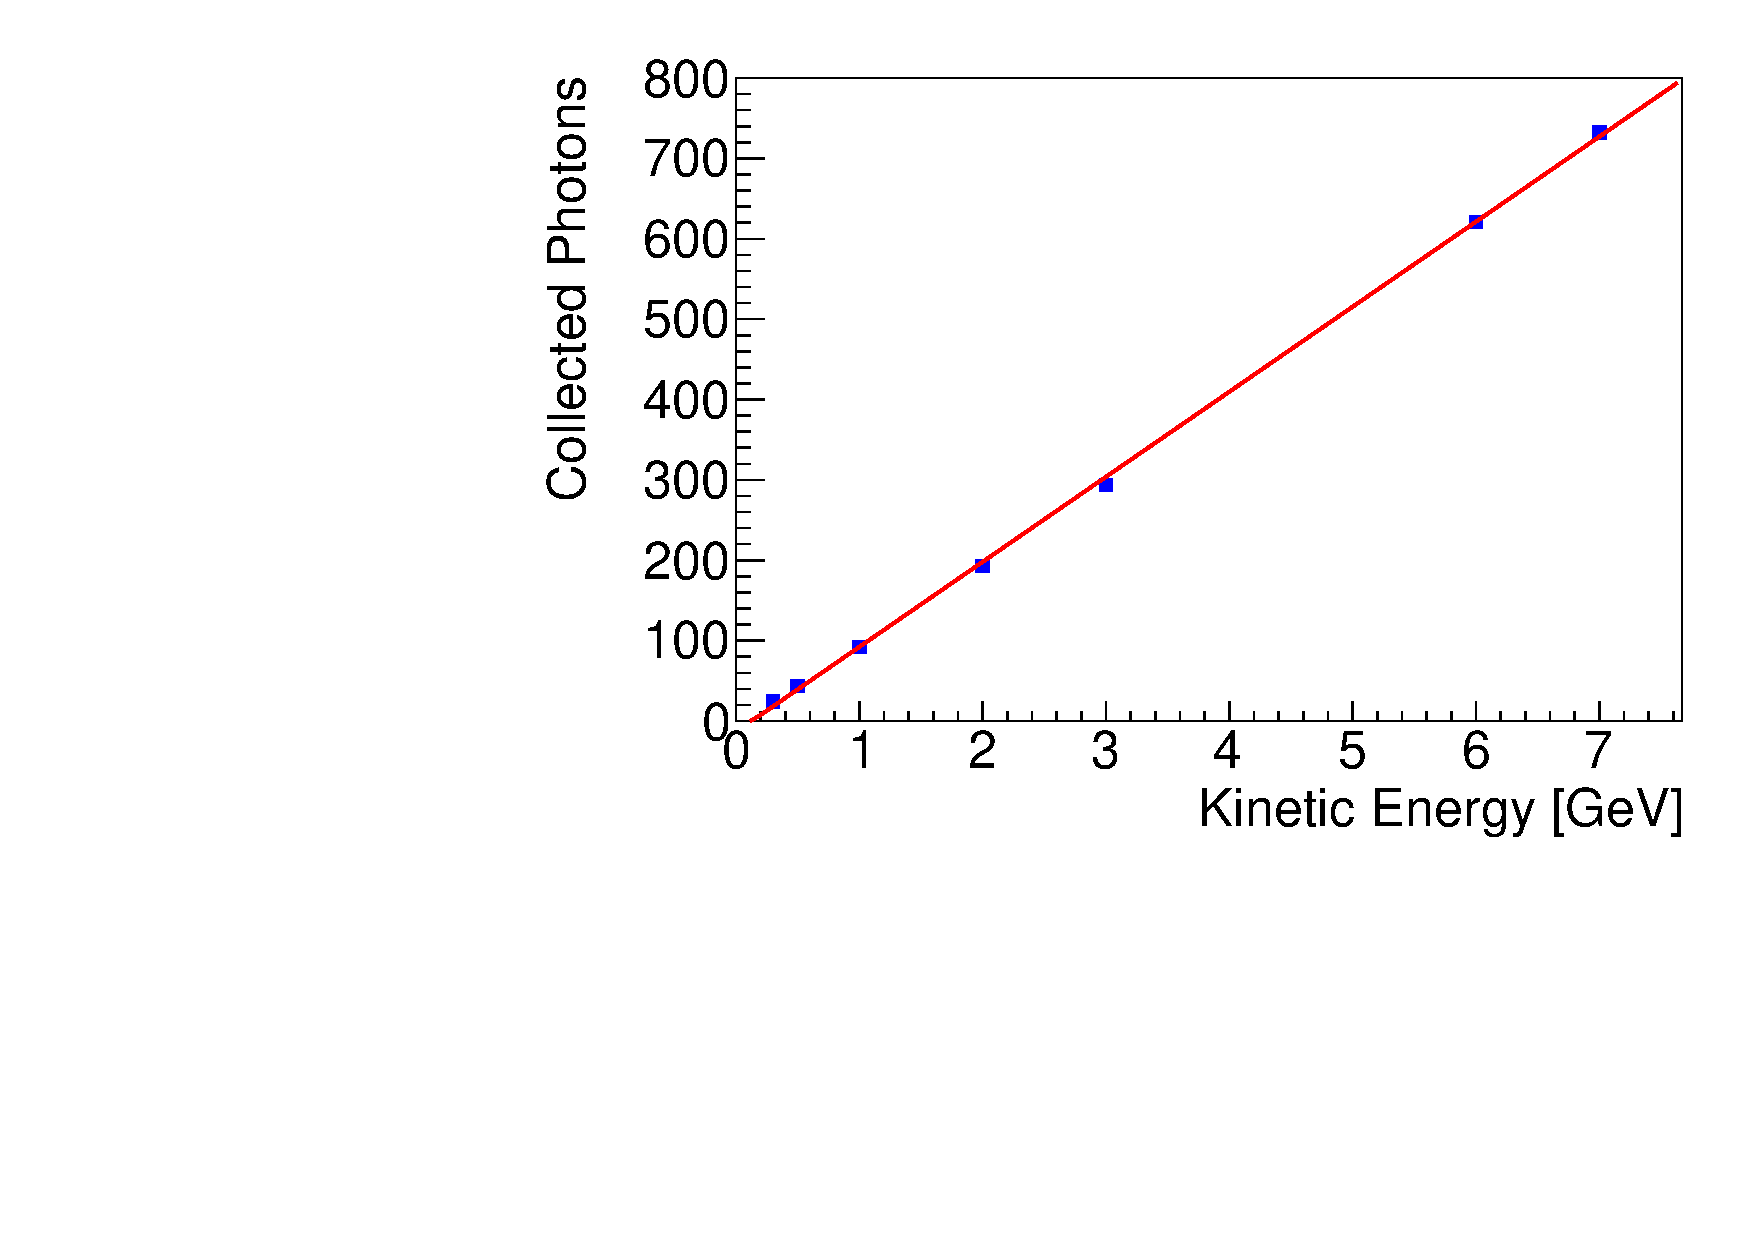
\includegraphics[width=0.45\linewidth]{pdsarapucabeamresponse.pdf}
\includegraphics[width=0.45\linewidth]{pdsarapucabeamresolution.pdf}

\end{dunefigure}

\begin{dunefigure}[Stability of the PD System during \dshort{pdsp} running]{fig:protodune-pds-stability}
{Stability of the \dword{sarapu} response in APA~6 measured with the UV-light calibration system (left) and the stability measurements of all \dword{pds} channels in APAs~4-6 with cosmic-ray muons tagged by the \dword{crt} (right).}
\includegraphics[width=0.5\linewidth]{pds-arapuca-lightvstime-daq-anorm.pdf}
\includegraphics[width=0.45\linewidth]{pds_daqside_tech_stability.pdf}
\end{dunefigure}

 
\subsection{Extended ARAPUCA (X-ARAPUCA)}
\label{sec:xarapuca-valid}


The \dword{xarapu} is an evolution of the \dword{sarapu} concept that moves the second wavelength-shifter from the inner surface of the dichroic filter to a wavelength-shifter doped plate that acts as a light guide. This design change was motivated by simulations that indicate a significant increase in collection efficiency for this configuration. 

In this section we describe in detail the first measurements that demonstrate the validity of the design, followed by several subsections that describe ongoing efforts to validate the final design.

\subsubsection{Single Cell \dword{xarapu} Measurements}
\label{sec:xarapuca-unicamp}

The first tests of an \dword{xarapu} cell were made at UNICAMP, Brazil, at the end of November 2018. 
The structure of the cell allowed it to operate as either an \dword{sarapu} or an \dword{xarapu}, with both single- or double-sided readout in both.  This flexibility will allow relative and absolute measurements of performance in the same cryostat and so provide a crucial step to validating the baseline design.

Building on the experience with the \dword{pdsp} prototypes, the frames for the test cell were fabricated from FR-4 G-10 in a configuration very similar to that planned for the \dword{fd} but with some small modifications necessitated by the requirements for holding a single window. The overall dimensions of the cell are \SI{12.3}{cm}$\times$\SI{10.0}{cm}$\times$\SI{1.56}{cm}. Figure~\ref{fig:xarapuca-cell} shows an exploded design drawing and the completed cell. 

\begin{dunefigure}[\dshort{xarapu} test cell]{fig:xarapuca-cell}
{\dword{xarapu} test cell:  Assembled cell (left); exploded model (right).  Note that exploded components can be duplicated on the back side (not shown) for double-sided test cell.} 
	\includegraphics[angle=270, origin=c, height=6.5cm]{pds-x-arapuca-test-cell-image-2}
	    \includegraphics[height=6.5cm]{pds-unicamp-single-cell-arapuca-exploded-r3}
\end{dunefigure}

The dichroic windows for the prototype are the same size as one of the six windows in a \dword{fd}-design \dword{xarapu} supercell: \SI{10.0}{cm}$\times$\SI{7.8}{cm}. The filter plate was coated with \dword{ptp} by vacuum evaporation (film thickness $\sim$ \SI{400}{${\mu}$g/cm$^2$})  using an in-house deposition system at \dword{unicamp} (see Figure \ref{fig:xarapuca-plates}). 
The thickness of the film needs to have a minimal value in order to ensure that the VUV light is fully absorbed. This minimum value is in the range of \SI{100}{${\mu}$g/cm$^2$} to \SI{200}{${\mu}$g/cm$^2$}. The  \SI{400}{${\mu}$g/cm$^2$} is chosen in order to ensure that the minimum thickness is reached everywhere on the filter even in presence of exceptional fluctuations (measured RMS of the order of \SI{30}{${\mu}$g/cm$^2$}). When the minimal thickness is reached the maximum conversion efficiency is obtained.

Adhesion was tested by submerging the coated filter in liquid nitrogen several times. The coating was visually inspected after each submersion, and no visible effect was observed. At the end of the test, the coated filter was weighed with a precision balance, and no loss of material was measured. The film was also analyzed with an optical microscope, and no signs of degradation could be observed. 

The wavelength shifting plate in the \dword{xarapu} configuration is made from Eljen EJ-286 blue WLS plate, with dimensions \SI{9.3}{cm}$\times$\SI{7.8}{cm}$\times$\SI{0.35}{cm}.  

The WLS plate thickness of \SI{0.35}{cm} was initially selected to optimize collection of light both by total internal reflection within the WLS plate and light trapped between the filter plates and the WLS plate.  Simulation has demonstrated that the detection efficiency performance of the detector reaches a shallow maximum at approximately this value.

The side walls of the test cell are lined with Vikuiti\texttrademark\ reflector, with cutouts at the positions of the photosensors.

\begin{dunefigure}[Coated dichroic filters and vacuum coating system]{fig:xarapuca-plates}
{Coated dichroic filter plates (left) and \dword{unicamp} thin film coating facility (right).} 
	\includegraphics[angle=90, height=6cm]{pds-coated-filter-plates-unicamp}\quad
	\includegraphics[height=8cm]{pds-unicamp-coating-machine}
\end{dunefigure}

The photosensors in the test cell are of the baseline type:  \SI{0.6}{cm}$\times$\SI{0.6}{cm} Hamamatsu S13360-6050VE \dwords{mppc}.  The photosensors are arranged in the same configuration as in the baseline design, with four \dwords{mppc} (passively ganged) mounted to two sides of the test cell, with positioning relative to the WLS plates and dichroic filters identical to the baseline design.  In a departure from the baseline design, the two passively ganged groups of four \dwords{mppc} are read out separately; no active ganging circuit is implemented for these tests. 

The test cell is installed at the bottom of a vacuum-tight stainless-steel cylinder (height $\sim$ \SI{30}{cm}) closed by two CF160 flanges and exposed to an alpha source\footnote{The same as used in the \dword{sarapu} proof-of-principle tests described in Section~\ref{sec:sarapuca-prototypes}.} 
placed at \SI{3}{cm} from the center of the dichroic window. Figure~\ref{fig:xarapu-teststand} shows photographs of the test cryostat and the test cell in the support structure; the alpha source holder is visible through the windows.
The stainless-steel cylinder  is deployed in a small open Dewar that is filled with commercial-grade LAr to act as a thermal bath.

\begin{dunefigure}[\dshort{xarapu} test stand]{fig:xarapu-teststand}
{Test cryostat (left) and \dword{xarapu} test cell mounting structure (right).  Note the alpha test source in holder.} 
	\includegraphics[height=6cm]{pds-unicamp-test-cryostat} \quad
	\includegraphics[height=7cm]{pds-unicamp-sample-cell-holder}
\end{dunefigure}  

The spectrum of the detected number of photons is shown in Figure~\ref{fig:xarapu-results} with a black line. The same fit procedure as in Section~\ref{sec:sarapuca-prototypes} allows an estimate of the number of detected photons for each alpha line. The result of the fit is shown with a red line in Figure~\ref{fig:xarapu-results}. Comparing the number of detected photons with the number of photons impinging on the \dword{xarapu} provides an estimate the global photon collection efficiency of the device as 3.5$\pm$0.5\%.
This result includes the correction for the crosstalk and afterpulsing of the two arrays of \dword{mppc} at their operating voltage.
The efficiency was stable for the duration of several days of this measurement.

The same test was repeated with the double-sided version of the \dword{xarapu}. Exactly the same set-up and the same device were used with the exception that the back plane coated with Vikuiti\texttrademark\ was replaced with a dichroic filter coated with \dword{ptp}. The same testing and analysis procedures were followed, and the global detection efficiency was found to be only 10\% less than the single sided version.   

\begin{dunefigure}[Alpha particle energy spectrum in an \dshort{xarapu} test cell]{fig:xarapu-results}
{Spectrum of the total number of \phel collected with the alpha source (blue line) fitted with the Monte Carlo prediction for the single-sided (left) and double-sided (right) \dword{xarapu}. Higher background activity at low energy was found for the second case.}

\includegraphics[height=6cm]{graphics/pds-alpha-fit-single.png}
\includegraphics[height=6cm]{graphics/pds-alpha-fit-double.png}
\end{dunefigure}  

The measured global collection efficiencies translate into an equivalent surface area\footnote{The equivalent surface area is defined as the product of the physical acceptance window of the device multiplied by its global collection efficiency.} of \SI{70}{cm$^2$} for a single sided \dword{xarapu} module and of \SI{63}{cm$^2$} for the double-sided, which exceed the specifications for our system by a substantial factor (Section~\ref{sec:fdsp-pd-simphys}). 

\subsubsection{ICEBERG Test Stand}
\label{sec:iceberg-teststand}

The \dword{iceberg} test-stand is a small-scale TPC, using smaller \dword{fd} \dword{apa} and cathode designs, constructed primarily to provide a platform for DUNE \dword{ce} testing at \dword{fnal}. 
The test stand consists of a \SI{94.7}{cm} $\times$ \SI{79.9}{cm} APA, with an approximately \SI{30}{cm} drift length to a cathode plane on each side (Figure~\ref{fig:fig-pds-iceberg-tpc}).  
It can accommodate up to two almost 1/2-length \dword{pd} modules\footnote{To enable the use of existing components for the \dword{apa} frame, the \dword{pd} modules are \SI{50}{mm} shorter than final modules, which required a slight modification to the \dword{pd} module design.} in a mounting structure nearly identical to the final DUNE FD configuration, allowing for testing of \dword{pd} prototype performance, electrical connections, and interfaces with the \dword{ce} and \dword{apa} systems (Figure~\ref{fig:fig-pds-iceberg-supercell}). 
In addition, the test stand will be used to allow comparisons between Mu2e-based warm electronics and \dword{pdsp} \dword{ssp} system, as well as testing newer versions of photosensors active ganging circuit designs.

The \dword{iceberg} facility will enable the primary validation of the \dword{xarapu} design prior to a full-scale test envisioned at a future \dword{pdsp} run in late 2021. 

At least three test campaigns are planned for the ICEBERG TPC with PD modules:  

\begin{enumerate}
    \item The initial photon detector configuration consisted of one full-length \dword{sarapu} supercell and one full-length \dword{xarapu} supercell.  Both of these supercells have single-side windows to allow comparisons of measurements with \dword{sarapu} and \dword{xarapu} prototypes in summer and fall 2018 \dword{pdsp}.  
    The first test run occurred in February-March 2019. This run demonstrated that both module prototypes and the cryogenic active ganging circuitry were operational and saw signals from both modules using a \dword{mu2e} front end electronics system modified for use by the \dword{dune} \dword{pd} (in a separate stream from the TPC \dword{daq}). Significantly, no crosstalk between the \dword{pd} and \dword{ce} readout electronics was observed.  Unfortunately, difficulties with the \dword{tpc} \dword{ce} and \dword{hv} systems prevented readout of ionization tracks required to allow direct comparisons between the PD modules and required the test to end before significant progress was made.

%\fixme{I modified the dates and goals for the second run dww 10/11/19}

    \item A second campaign is planned for late July through December 2019. It uses the same photon detector modules as the first campaign but will provide comparison of data from the \dword{sarapu} and \dword{xarapu} modules with cosmic ray tracks measured in the \dword{tpc}.  These tracks will facilitate comparisons of \dword{ssp} and \dword{mu2e} readout systems for similar events as indicated by \dword{tpc} tracking, as well as additional \dword{pd} and \dword{ce} crosstalk checks.  Two short runs (ICEBERG 2A and 2B) occurred in August and September 2019, during which the DaPHNE and SSP were commissioned and initial photosensor bias voltage studies were conducted.  These runs were cut short due to problems with the cryogenic filtering system for the \dword{iceberg} cryostat,  Run 2C is scheduled for late October/early November 2019, during which we expect to achieve our goals of matching \dword{tpc} tracks to flashes observed in the PD.

    \item A third campaign is planned for spring of 2020.  This run (ICEBERG run 3) will incorporate two \dword{sarapu} and two \dword{xarapu} supercells, though it is partially occluded in the frame due to the limitations in \dword{apa} size mentioned above.  One supercell of each kind will be single-sided and one double-sided, allowing for additional comparisons of \dword{pd} technologies.  This campaign will also demonstrate readout of \dword{mu2e} electronics by the \dword{iceberg} \dword{daq}.  In addition, we plan to incorporate a prototype of the \dword{dune} \dword{sp} monitoring system.
    
\end{enumerate}

The test stand will provide testing and validation of the \dword{pds} Mu2e-based electronics system, including a side-by-side comparison with the \dword{pdsp} \dword{ssp} electronics readout. In addition, concurrent data taking with the TPC and light collection system will allow us to study TPC-induced noise on the \dword{pd}, \dword{pd}-induced noise on the TPC, grounding scheme configuration, controller-\dword{daq} and controller-\dword{feb} interfaces, bandwidth and rates issues, online and offline \dword{pd}-TPC interfaces, zero-suppression techniques, firmware development, accepting and producing triggers, and, in general, will inform possible upgrade paths for the system. 


\begin{dunefigure}[ICEBERG TPC model and assembled \dshort{apa}]
 {fig:fig-pds-iceberg-tpc}
 {Solid model of ICEBERG TPC (left), and assembled ICEBERG \dword{apa} (right).  Note the two sets of \dword{pd} module mounting rails, which are vertical in this image but horizontal during operation. The centrally-mounted \dword{apa} allows for testing of double-sided readout photon detector modules.}
\includegraphics[angle=0,height=6.5cm]{pds-iceberg-tpc}
\includegraphics[angle=0,height=6.5cm]{pds-iceberg-apa.pdf}
\end{dunefigure}

\begin{dunefigure}[Single supercell ICEBERG PD module]
 {fig:fig-pds-iceberg-supercell}
 {Software solid model of a single supercell ICEBERG PD module (left) and fabricated components during assembly (right).  The connector board (green) in the right photo is mounted to the \dword{apa} frame prior to wire wrapping.}
\includegraphics[angle=0,height=6.5cm]{pds-iceberg-run-1-module.pdf}
\includegraphics[angle=0,height=6.5cm]{graphics/pds-iceberg-module-assembly-photo.pdf}
\end{dunefigure}

Delays in the \dword{iceberg} commissioning schedule unrelated to the \dword{pdsp} system prevented having significant results available in time for this TDR. However, test stand data are still expected to provide critical input for the 60\% design review in late 2019. Additional runs in 2020 will assist in preparing for the final design review and \dword{pdsp2} module designs.


\subsubsection{SBND}
\label{sec:valid-sbnd}

The baseline photon detector system for the SBND experiment includes three types of detector:  TPB-coated cryogenic photomultipliers, an array of dipped light-collector bars similar to those used in \dword{pdsp}, and a small array of \dword{xarapu} modules.  Eight modified \dword{xarapu} modules will provide an opportunity for a long-term system test of a significant number of key components prior to the \dword{sbnd} \dword{pds} \dwords{prr}.  Each \dword{sbnd} \dword{xarapu} will consist of two dichroic filter plates with dimensions \SI{100}{mm}$\times$\SI{78}{mm}$\times$\SI{1.5}{mm}
 that are coated with \dword{ptp} at the \dword{unicamp} vacuum deposition facility.  These filters will be produced by Opto Electronics S.A. in Brazil, the leading vendor candidate for the \dword{dune} \dword{pd} modules.  Also, each \dword{sbnd} module will contain an Eljen \dword{wls} plate  
\SI{200}{mm}$\times$\SI{78}{mm}$\times$\SI{4}{mm}. FR-4 G-10 frame components will be fabricated at local vendors, representing candidates for eventual \dword{dune} fabrication.  A software solid model of the design is shown in Figure~\ref{fig:fig-SBND-modules}.

The eight \dword{sbnd} \dword{xarapu} modules will be assembled at \dword{unicamp} using the \dword{dune} \dword{pd} consortium assembly plan,
which will provide valuable experience with fabrication of multiple modules at that site.

%\fixme {X-ARAPUCAs in SBND now settled. dww 10/11/19}

In the summer of 2019, the \dword{sbnd} collaboration re-opened the question of the composition of their light collection system, eliminating the dipped bar modules in favor of \num{200} additional \dword{xarapu} modules.  These modified modules will use WLS plates and coated filter plates identical to those proposed for \dword{dune}, and frame components very similar to those in the final \dword{dune} \dword{pd} system.  The modification to the \dword{sbnd} system will provide a larger scale, long-term test of critical \dword{pd} components and will significantly enhance the value of the test as a development run for the \dword{unicamp} facility.

%\fixme {delayed the dates here, too! dww 10/11/19}

Module assembly for \dword{sbnd} will be complete by the end of CY 2019, with installation in the detector beginning in November 2019.  Filling with \dword{lar} and operation will occur in summer 2020, and we expect initial results from the \dword{pd} system in fall 2020.  \dword{sbnd} will be the first large-scale operational testing for \dword{xarapu} modules very similar to those to be used in \dword{dune}.
\dword{sbnd} will also use coated reflector foils, which will provide additional valuable information on that \dword{dune} \dword{pds} option.  

While not part of the \dword{dune} project, and not part of the validation schedule for the \dword{pdsp}, \dword{sbnd} results will inform our preparations for the final design review of these components and the fabrication of modules for \dword{pdsp2}.  

\begin{dunefigure}[SBND \dshort{xarapu} Modules]
 {fig:fig-SBND-modules}
 {Software solid model of two-cell \dword{xarapu} modules for SBND, exploded (left) and assembled (right).}
\includegraphics[angle=0,width=8.4cm,height=5.5cm]{graphics/pds-sbnd-xarapu-exploded.pdf}
\includegraphics[angle=0,width=8.4cm,height=5.5cm]{graphics/pds-sbnd-xarapu-assembled.pdf}
\end{dunefigure}

\subsubsection{\dword{pdsp2}}
\label{sec:valid-pdune2}

Following completion of the initial run of \dword{pdsp}, a second test run called \dword{pdsp2} is planned in the same cryostat.  This test will serve as a final validation of all pre-production \dword{spmod} detector designs, verifying their performance and ensuring they perform in concert with no interference.  We intend to replace three complete \dword{apa} assemblies with pre-production modules to allow testing \num{30} final design \dword{pd} modules.  

\dword {pdsp2} will allow for the first end-to-end test of the final \dword{pd} system, with significantly re-designed elements:
\begin{itemize}
    \item full-size \dword{xarapu} modules read out in conjunction with a \dword{tpc};
    \item \num{48}-channel photosensor active ganging;
    \item final design electrical connectors for PD modules mounted inside full-scale \dword{apa}s;
    \item pre-installed cable harnesses inside \dword{apa}s including final module supports;
    \item readout of full-scale \dword{xarapu} modules using modified \dword{mu2e} electronics, including integrating \dword{tpc} and \dword{pd} event matching into the \dword{daq} system.
\end{itemize}

Two candidate photosensors will be tested (\num{15} modules built with each sensor type), and the experience gained while fabricating \dword{pdsp2} will be an important factor for selecting 
%one of the main factors used to either select 
between the candidate sensors or deciding to incorporate both in the \dword{pds} final design.  All other components will be final design components, so at least half of the \dword{pd} modules in \dword{pdsp2} will represent ``Module 0'' level of design. 

While all of these elements will have been tested previously individually and/or at smaller scale, \dword{pdsp2} will represent the final pre-production testing of all the final design components as an integrated system.

The schedule for \dword{pdsp2} calls for \dword{pd} modules to be installed into \dword{apa} modules at \dword{cern} in the spring of 2021. However, some components, including module support rails, electrical connectors, and cable harness components, must be mounted inside \dword{apa} frames prior to wire wrapping and so must be available by mid-2020.

Re-filling of the \dword{pdsp} cryostat will begin in the fall of 2021, with operations beginning in late 2021.  Operation of \dword{pdsp2} will continue for at least one year.  This schedule allows for initial operation of the complete system prior to the \dword{pd} \dword{prr} and the beginning of mass-production of \dword{sp} modules in summer 2022, although some components (including dichroic filter plates and photosensors) will have begun procurement by that time.  These components are physically smaller and more amenable to testing in smaller cryostats, reducing the exposure due to this delay.  These scheduling issues will be addressed in more detail in \ref{sec:fdsp-pd-org-cs}.

If the decision has been taken to proceed with our performance enhancement alternates (xenon doping or CPA-mounted reflector foils, see Section\ref{sec:fdsp-pd-enh}), they will be tested in \dword{pdsp2} as well.

\subsubsection{Long Term Cryogenic Aging}
\label{sec:valid-longtermaging}

It is difficult to accelerate aging effects due to long-term immersion of components in cryogenic liquids.  While mechanical aging due to thermal expansion/contraction can be readily accelerated by cycling the components to be tested through multiple cycles, long term aging not related to rapid thermal stresses are not amenable to easy acceleration.  An example of such a process might be dissolution of \dword{ptp} coatings over time.

Mitigation of these risks involves some level of long-term exposure to liquid cryogen with extrapolation to the DUNE timescales.  Several such tests are planned for the PD system:

%\fixme{added some delays here, too! dww 10/11/19}

\begin{itemize}

    \item \dword{pdsp} will provide a long-term test of two \dword{sarapu} modules for a period of up to one year at the time of draining in the Winter of 2020.  The system will be continuously monitored for gain and response of the detectors, and will provide information regarding aging of FR-4 G-10 structures, photosensors, and coated filter plates.  Other \dword{pdsp} detectors (Double-shift bar designs) will give some indication of aging of similar \dword{wls} plates to those used in the \dword{xarapu} modules.

    \item \dword{sbnd} will provide a multi-year test of many X-ARAPUCA components, such as coated filter plates, \dword{wls} plates, and photosensors.  \dword{sbnd} will run for at least three years, starting in late 2020.  As part of a running experiment, the system will be continuously monitored for gain and response of the detectors and will provide information regarding aging of FR-4 G-10 structures, photosensors, and coated filter plates as well as \dword{wls} plates to be used in the \dword{xarapu} modules.
    
    In addition, TPB-coated reflector foils will be tested in \dword{sbnd}. While coated reflector foils are not part of the baseline PD system, this will provide validation for the concept we currently present as an option (Section~\ref{sec:fdsp-pd-enh-cathode}).
    
    \item \dword{pdsp2} will provide a long term test of full-scale \dword{xarapu} modules in the final \dword{dune} configuration. While this test will begin shortly before \dword{dune} \dword{pd} module production fabrication, it will provide long-term validation of all \dword{xarapu} components during module production prior to integration into the \dword{apa} frames, allowing for possible insights and improvements into the \dword{xarapu} design.

\end{itemize}


\subsection{Materials Selection, Testing and Validation}

\subsubsection{\dword{pd} Module Mechanical Frame}

The APA mechanical frame components are fabricated from FR-4 G-10 (Garolite\textregistered), a glass-epoxy laminate commonly used in printed circuit boards and other mechanical applications where an electrically insulating component with low thermal expansion coefficient is required.  G-10 is widely used in cryogenic applications, including most of the other \dword{dune} subsystems (See \citedocdb{10452} for an extensive discussion in the context of the HV system cathode planes). 
FR-4 has been certified at the \dword{fnal} materials test stand as an acceptable material for use in \dword{dune} from the standpoint of \dword{lar} contamination.

Thermal contraction of FR-4 is similar to that of stainless steel, simplifying design of the module interface with the \dword{apa} frame.
It allows us to use long printed circuit boards for routing photosensor electrical signals along the detector sides without incurring thermal expansion issues.  As an excellent insulator, it simplifies electrically isolating the PD system from the \dword{apa} frame, as required by the \dword{dune} grounding scheme.
However, selecting FR-4 as our main module structural material comes at the cost of some additional difficulty machining components.

All fasteners used in the \dword{pd} are stainless steel alloy 304, widely used in cryogenic applications.  This alloy has also been certified at the \dword{fnal} materials test stand as an acceptable material for use in \dword{dune} from the standpoint of \dword{lar} contamination.

\subsubsection{\dword{pd} Module-\dword{apa} Frame Mechanical Support Structure}

All \dword{pd} mechanical supports (including rails, brackets and fasteners are to be manufactured from stainless steel alloy 304.  This has the benefit of matching thermal contraction coefficients with the \dword{apa} frame and being approved for use in \dword{lar} by the materials test stand.

\subsubsection{Dichroic Filter/Filter coating}

The dichroic filters used in \dword{xarapu} consist of a fused silica substrate, coated on one face to provide the required dichroic properties and on the opposite face with a thin evaporated layer of \dword{ptp}.
Fused silica was selected in part due to its excellent low-temperature properties.  It is widely used as an optical window in low temperature applications, due to its stability and low coefficient of thermal contraction; fused silica dichroic filters have performed well in many \dword{sarapu} validation tests.

Stability of the \dword{ptp} coating is of greater concern.  Initial validation of the \dword{sarapu} in \dword{tallbo}, \dword{pdsp}, and in repeated cryogenic immersion tests at \dword{fnal} and other facilities has demonstrated that while it is possible to generate highly-reliable \dword{ptp} coatings on fused silica substrates, careful surface preparation and deposition procedures are required to prevent failure of the coating.  
Dissolution of similar wavelength-shifting coatings into liquid argon has been reported but in a technology-dependent fashion~\cite{Asaadi:2018ixs}, so continued investigation of the design specific to \dword{dune} is necessary to confirm robustness. 


A test stand has been developed at Syracuse University to investigate the long-term stability of \dword{xarapu} optical coatings in liquid argon that will
subject coated materials to a continuous flow. This will stress the adhesion of the coating to the plates to simulate the convective flow of liquid argon in the far detector cryostat.
 
The test stand consists of a \SI{74}{L} liquid argon cryostat with a frame suspending coated filters beneath an impeller driving a continuous flow of liquid argon across them. Filters will be inspected monthly for degradation in their opacity, transparency, and wavelength-shifting response. A dark box containing a visible-light and near-UV scanning bed will measure wavelength shifting performance of the tested elements before and after suspension within the argon flow.

%\fixme{ delay...dww 10/11/19}

Testing will begin in late 2019, when coated filter plates become available, and is expected to run through late 2020.

\begin{dunefigure}[\dshort{pds} coating test stand]
 {fig:pds-CoatingTestStand}
 {Two components of the \dword{pd} coating test stand. (1) VUV monochromator (foreground) and 2-axis scanning chamber (background) 
 %at Syracuse University, USA, 
 currently undergoing recommissioning (left); and (2) solid model of \SI{74}{L} liquid argon cryostat for quality control studies and future detector development (right).}
\includegraphics[angle=0,height=6.cm]{pds-su-vuv-monochromator.jpg}
\hspace{0.02\textwidth}
\includegraphics[angle=0,height=6.cm,trim={2.2in 0.75 2.2in 0.75},clip]{pds-su-coatingteststand.png}
\end{dunefigure}


\subsubsection{\dword{wls} plates}

The \dword{xarapu} wavelength shifting plates are fabricated by the same vendor as the light guide bars utilized in the double-shift \dword{pdsp} modules.  The plates are made with the same transparent matrix material, but have a different wavelength shifting dopant chosen to provide a better match to the spectral sensitivity of the PD SiPM (around \SI{430}{nm}). It also has an emission spectrum very similar to TPB, used in the standard ARAPUCA, which ensures the same performance of the dichroic filter and of the reflective coatings.

While it is possible that the cryogenic properties of this modified \dword{wls} material may be altered by the change in doping agent, it is expected that the tests done for the double-shift bar prototypes are a valuable guide for their expected performance.  As part of the design verification, samples of these bars were manually thermocycled to verify they didn't craze. In addition, we used a LAr test stand 
with an alpha source behind a small sample of the \dword{wls} plate to scan the attenuation length of a short sample. Finally, we built a darkbox with a $\sim\,$\SI{420}{nm} LED scanning down the length of a full bar to verify the attenuation length and to compare the results to the LAr data. (This formed the basis of the threshold requirements on in-air attenuation length measurement for the \dword{pdsp} batch.) 
This same sequence will be undertaken for the light guides selected for \dword{xarapu}. 

As with most other components, it is not possible to simulate long-term exposure to \dword{lar} of a length similar to that expected in \dword{dune} operation, but we will substitute continuous long term exposure by running samples through repeated thermal cycling to maximize thermal stresses in the material.  Finally, samples of the \dword{wls} plates will be certified for use in \dword{dune} in the materials test stand at \dword{fnal}.  


%%%%%%%%%%%%%%%%%%%%%%%%%%%%%%%%%%%%%%%%%%%%%%%%
% Provided by dj 11/26/18
\subsection{Calibration and Monitoring}
\label{sec:fdsp-pd-validation-candm}

All major components of the \dword{spmod} \dword{pds} calibration and monitoring system have been designed, fabricated, tested, and operated in \dword{pdsp}. Figure~\ref{fig:pds_calmon_hw_photo} shows the hardware components of the system.
Although at a longer wavelength (\SIrange{245}{280}{nm}) than \lar scintillation light (\SI{127}{nm}), the UV light from the calibration system exercises the full chain of measurement steps initiated by a physics event in the \dword{detmodule}, starting from the wavelength conversion, photon capture in the \dword{sarapu}, photon detection, and the \dword{fe} electronics readout.

A substantial \dword{pdsp} data set has been collected and the data analysis is underway. 
Goals of the analysis are to verify that the \dword{cpa} includes an optimal distribution of light diffusers for the \dword{spmod};
to demonstrate capability of the system evaluate gain and timing resolution; to perform relative comparisons of photon channels;
and to characterize and monitor stability of the \dword{pds} over the duration of \dword{pdsp}. Here we present preliminary results that demonstrate the timing performance of the system, the stability of the two types of \dword{sipm}, and the photon detection rate over several months.

%and will inform the design of an optimal \dword{pds} calibration and monitoring plan for the \dword{spmod}.

\begin{dunefigure}[\dshort{pdsp} UV calibration and monitoring system]
 {fig:pds_calmon_hw_photo}
 {The photographs show the hardware components of the \dword{pdsp} calibration and monitoring system.}
% \includegraphics[angle=0,width=11.4cm,height=9cm]{graphics/pds-calmon-fig2.png}
 \includegraphics[angle=0, height=9cm]{graphics/pds-calmon-fig2.png}
\end{dunefigure}


Figure~\ref{fig:pds_calmon_timing} (left) shows a typical double waveform recorded by an \dword{pdsp} \dword{ssp} module as a response to calibration system
light pulses illuminating an \dword{sarapu} channel; the figure on the right demonstrates that the calibration system has the precision and stability to meet the system requirements.

Figure \ref{fig:pds-calmon-charge-avalanche} shows the \dword{sipm} gain (charge per \phel-induced avalanche) extracted from the calibration data normalized to the average gain during the period. The left figure shows the results over a period of three months for the MPPCs mounted on the \dword{sarapu} modules; the right figure shows the results over a period of six months for the SensL \dwords{sipm} that are mounted on a set of double-shift and dip-coated light collector bars. The colors correspond to different readout channels for the left figure and to the average of the sensors in PD modules for the right figure.
All sensors are stable at the level of a few percent, with no significant systematic decline.

Figure \ref{fig:pds-calmon-photons-apa6} shows the measured signal (average number of photons, normalized to the average signal over the three-month period) from the double-shift and dip-coated light collector bars in APA~6 that are read out with MPPC \dwords{sipm} (left), and those in APA~4 that are read out with SensL \dwords{sipm} (right), in response to the calibration flashes. The colors correspond to the average of the sensors in PD modules. The measured signal is sensitive to stability in the intensity of the calibration system light and the response of the light collectors (including effects such as changes in wavelength shifter properties and \dword{sipm} response). The ratio is stable at the few percent level.

These results verify operation and performance of both the \dword{pds} and the UV-light calibration system. This monitoring will continue for the duration of the \dword{pdsp} operation.

\begin{dunefigure}[\dshort{pdsp} \dshort{sarapu} response to UV calibration and monitoring system]
 {fig:pds_calmon_timing}
 {Double waveforms recorded by \dword{pdsp} \dword{ssp} as a response to calibration system light pulses collected by an \dword{sarapu} channel (left). Distribution of measured times of the first light pulse in the two-pulse waveform for 1000 pulse pairs (right).}
  \includegraphics[height=5.8cm,width=0.45\linewidth]{graphics/pds-double-waveform-arapuca-example.pdf}
 \includegraphics[height=6cm,width=0.45\textwidth]{graphics/pds-example-t1.pdf}  \end{dunefigure}

\begin{dunefigure}[\dshort{pdsp} gain monitoring with UV calibration and monitoring system]
 {fig:pds-calmon-charge-avalanche}
 {Normalized gain measurements using the calibration system light pulses: MPPC \dwords{sipm} on the \dword{sarapu} modules (left); SensL \dwords{sipm} on the dip-coated and double-shift bars in APA~3 (right). This demonstrates the stability of the gain for both types of device operating in \lar.}
% The following are the MPPC  Charge/Avalanche from Dante 7/17/19
  \includegraphics[height=5.5cm,width=0.48\textwidth]{graphics/pds-arapuca-calibration-stability.pdf}
% The following are the SensL Charge/Avalanche from ChrisM 7/17/19
  \includegraphics[height=5.5cm,width=0.48\textwidth]{graphics/pds-avg-mean-adc-led-apa3-sensl.pdf}
\end{dunefigure}

\begin{dunefigure}[\dshort{pdsp} UV calibration and monitoring system stability]
 {fig:pds-calmon-photons-apa6}
 {Measurement of the signal from the calibration system using the dip-coated and double-shift bars in APA~6 that have MPPC \dwords{sipm} (left) and in APA~4 that have SensL \dwords{sipm}. The signal is normalized to the average response over the entire period.
 }
  \includegraphics[height=5.5cm,width=0.48\textwidth]{graphics/pds-avg-mean-adc-led-apa6-mppc.pdf}
% The following are the APA4 SensL Normalized Light Yield from ChrisM 7/17/19
  \includegraphics[height=5.5cm,width=0.48\textwidth]{graphics/pds-avg-mean-adc-led-apa4-sensl.pdf}

\end{dunefigure}